% Configurazione della pagina
\documentclass[
  12pt,
  a4paper,
  headings=optiontoheadandtoc
]{scrreprt}
\setlength{\parskip}{\baselineskip}
%\pagenumbering{gobble}

% Dichiarazione dei pacchetti utilizzati
\usepackage{ragged2e}
\usepackage{tabularx}
\usepackage{graphicx}

% Metadati per il titolo
\author{Ghellere Nicolò (VR486914), Milli Manuel (VR488346),\\Sacchetto Riccardo (VR485898)}
\date{15 febbraio 2023}
\title{Dispositivo di gestione di un parcheggio}
\subtitle{Elaborato SIS - Relazione}

% Cartella delle immagini
\graphicspath{ {./img/} }


% ===== Inizio del documento =====
\begin{document}

% Creazione del titolo
\maketitle

% Configurazione e creazione della ToC
\renewcommand*\contentsname{Indice}
\tableofcontents
\newpage

\chapter[nonumber=true]{Architettura del dispositivo}

Lo scopo del dispositivo descritto in questa relazione e realizzato sotto forma di circuito digitale in formato BLIF per SIS è quello di gestire un parcheggio con ingresso e uscita automatizzati, ricevendo in input l'azione dell'utente (ingresso o uscita) e il settore d'interesse (A, B o C) e aprendo la sbarra d'ingresso o uscita a patto che il settore selezionato non sia, rispettivamente, pieno o vuoto.

L'input è costituito da cinque bit: due per l'azione (ingresso=01, uscita=10) e tre per il settore (A=100, B=010, C=001); l'output è invece costituito da sei bit: uno che rappresenta la scelta di un settore non valido, due che comunicano quando aprire la sbarra d'ingresso (10) o quella d'uscita (01) e tre che segnalano i settori pieni (il primo per A, il secondo per B e il terzo per C).

I due componenti logici del dispositivo sono la FSM con i cinque stati che rappresentano le fasi del ciclo di funzionamento e il datapath che si occupa di memorizzare, aggiornare e analizzare la quantità di veicoli nei vari settori, tenendo conto che in A e B ci possono essere fino a un massimo di 31 veicoli e in C un massimo di 24.

\section[nonumber=true]{Il controller}

La FSM che funge da controller per il circuito di controllo del parcheggio presenta cinque stati diversi:

\begin{itemize}
  \item \textbf{OFF}: Rappresenta lo stato d'inattività del dispositivo. Finchè si trova in questo stato il circuito attenderà la sequanza di avvio \textbf{11111} ignorando ogni altro input e ponendo a 0 ogni bit di output
  \item \textbf{READA}: Primo stato di avvio. L'input ricevuto in questo stato verrà interpretato come il numero di veicoli posizionatisi nel settore A durante l'inattività del sistema di controllo
  \item \textbf{READB}: Secondo stato di avvio. L'input ricevuto in questo stato verrà interpretato come il numero di veicoli posizionatisi nel settore B durante l'inattività del sistema di controllo
  \item \textbf{READC}: Terzo stato di avvio. L'input ricevuto in questo stato verrà interpretato come il numero di veicoli posizionatisi nel settore C durante l'inattività del sistema di controllo
  \item \textbf{RDY}: Normale stato di funzionamento. Finchè si trova in questo stato il dispositivo risponderà alle richieste d'ingresso o uscita degli utenti, alzando e abbassando le sbarre e comunicando i settori pieni. Il sistema tornerà nello stato \textbf{OFF} quando riceverà la squenza \textbf{00000}
\end{itemize}

Internamente, al fine di comunicare con il datapath e di controllarne il funzionamento la FSM utilizzerà i seguenti segnali:

\begin{itemize}
  \item \textbf{WA}: Segnala al datapath quando interpretare l'input come numero di posti occupati in A durante la notte. Posto a 1 solo in \textbf{READA}
  \item \textbf{WB}: Segnala al datapath quando interpretare l'input come numero di posti occupati in B durante la notte. Posto a 1 solo in \textbf{READB}
  \item \textbf{WC}: Segnala al datapath quando interpretare l'input come numero di posti occupati in C durante la notte. Posto a 1 solo in \textbf{READC}
  \item \textbf{OPENPARKS}: Segnala quando il dispositivo è pronto a ricevere le query degli utenti aprendo le sbarre in risposta a esse. Posto a 1 da \textbf{RDY}
  \item \textbf{SHOWFULLA}: Segnala al datapath quando mostrare se il settore A è pieno. Posto a 1 da tutti gli stati consecutivi a \textbf{READA}
  \item \textbf{SHOWFULLB}: Segnala al datapath quando mostrare se il settore B è pieno. Posto a 1 da tutti gli stati consecutivi a \textbf{READB}
  \item \textbf{SHOWFULLC}: Segnala al datapath quando mostrare se il settore C è pieno. Posto a 1 da tutti gli stati consecutivi a \textbf{READC}
  \item \textbf{INVSEC}: Mappato al primo bit dell'output generale, segnala quando l'utente ha immesso un settore non valido. Può essere posto a 1 da \textbf{RDY}
\end{itemize}

Per meglio comprendere il funzionamento del controller segue il digramma degli stati della FSM che lo costituisce. I bit di input sono elencati come da specifica mentre quelli di output sono nell'ordine descritto dall'elenco appena riportato:

\Centering
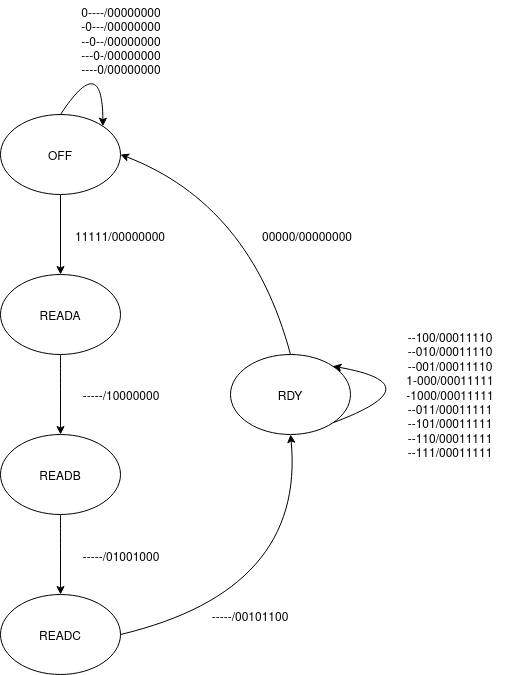
\includegraphics[scale=0.75]{controller}

\RaggedRight

\section[nonumber=true]{Il DataPath}

\Centering
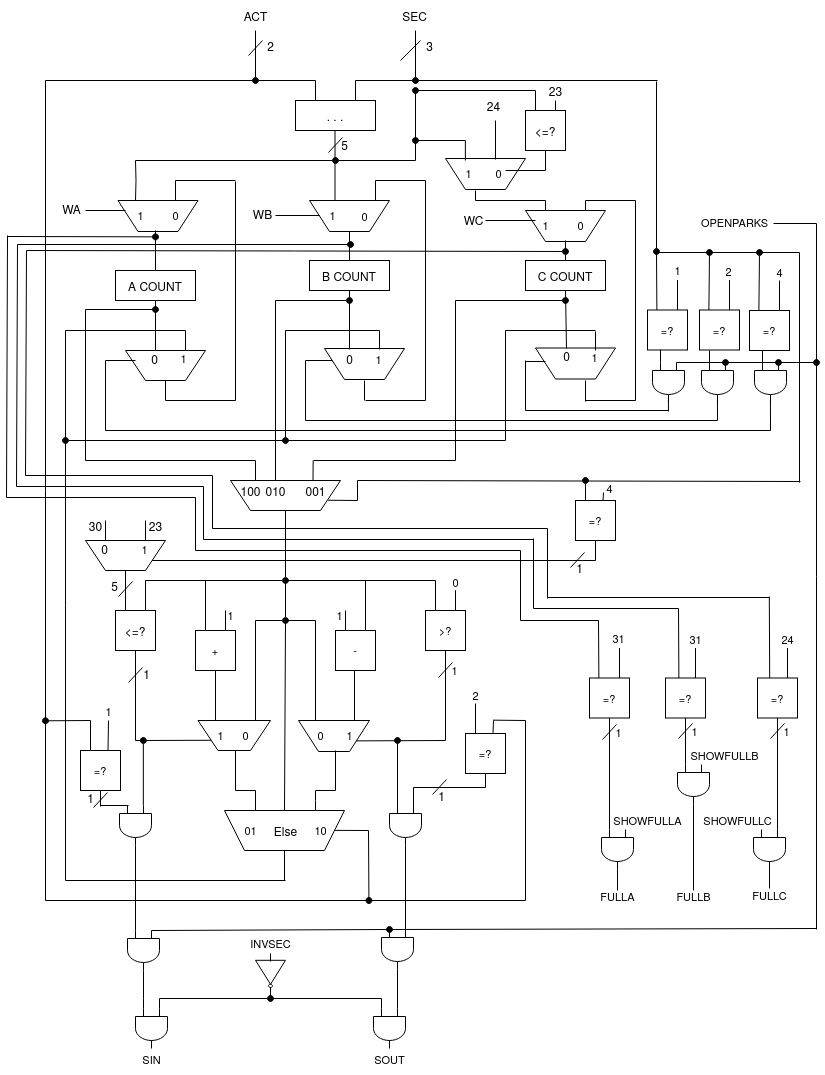
\includegraphics[scale=0.5]{datapath}

\RaggedRight

Come è possibile notare osservando il diagramma riportato, il datapath è composto da due parti principali: la logica di caricamento e di gestione dei registri e la logica di aggiornamento del conteggio.

Le due parti sono separate dal one-hot multiplexer a tre ingressi collocato al centro del diagramma, il quale riceve in input tutti e tre i conteggi salvati al ciclo precedente e trasmette alla logica di calcolo solo quello che corrisponde al parcheggio d'interesse dell'utente.

\subsection[nonumber=true]{Gestione dei registri}

Il datapath presenta tre registri separati, i quali contengono i conteggi dei veicoli parcheggiati nei vari settori. Ogniuno di questi può ricevere in ingresso, in base allo stato del sistema, tre diversi valori:

\begin{itemize}
  \item l'input dell'utente, qualora il controller sia nella fase di ricezione dei valori immessi dall'operatore;
  \item il precedente valore del registro, qualora l'operatore non stia immettendo un nuovo valore e l'utente non stia entrando o uscendo dal relativo settore;
  \item il valore aggiornato dalla logica di calcolo qualora si sia verificato un ingresso o un'uscita.
\end{itemize}

La scelta del valore da fornire in ingresso a ogni registro è operata da due multiplexer per ciascuno, uno dei quali seleziona (visto il \textbf{SEC} su cui sta operando l'utente) se caricare in feedback l'output della logica di calcolo al posto del vecchio valore e uno che, sulla base del segnale \textbf{Wx}, decide se caricare tale valore di feedback o quello presente in input.

\subsection[nonumber=true]{Logica di calcolo e aggiornamento}

Come già accennato, quando l'utente specifica in input in/da quale settore vuole entrare/uscire, un one-hot multiplexer trasferisce sul proprio output il conteggio dei posti occupati in tale settore. Il valore verrà quindi trasmesso a un sommatore (che lo incrementa di 1) e a un sottrattore (che lo decrementa di 1), i cui risultati potranno essere utilizzati per il segnale di feedback. Quest'ultimo, in particolare, assumerà diversi valori in base ad alcune condizioni:

\begin{itemize}
  \item Se il vecchio conteggio è minore del massimo numero di posti occupabili nel settore scelto e l'azione è ingresso, il feedback sarà il risultato dell'incrementatore
  \item Se il vecchio conteggio è maggiore di 0 e l'azione è uscita, il feedback sarà il risultato del decrementatore
  \item In tutti gli altri casi, il feedback sarà uguale al vecchio conteggio
\end{itemize}

Per quanto riguarda gli output generali,
\begin{itemize}
  \item \textbf{SIN} (il segnale di controllo della sbarra d'ingresso) sarà posto a 1 se il vecchio conteggio è minore del massimo numero di posti occupabili nel settore scelto, l'azione è ingresso e \textbf{OPENPARKS} è 1;
  \item \textbf{SOUT} (il segnale di controllo della sbarra di uscita) sarà posto a 1 se il vecchio conteggio è maggiore di 0, l'azione è uscita e \textbf{OPENPARKS} è 1;
  \item i tre bit che segnalano i settori pieni saranno invece posti a 1 rispettivamente se \(\textbf{ACOUNT}=31 \wedge \textbf{SHOWFULLA}\), \(\textbf{BCOUNT}=31 \wedge \textbf{SHOWFULLB}\), \(\textbf{CCOUNT}=24 \wedge \textbf{SHOWFULLC}\).
\end{itemize}

\chapter[nonumber=true]{Misure e statistiche}

\section[nonumber=true]{Statistiche pre e post ottimizzazione}

Si riportano di seguito le statistiche riguardanti il circuito nel suo stato pre e post ottimizzazione.

I valori ottimizzati riportati qui sotto sono stati ottenuti eseguendo per tre volte lo ``script.rugged'', procedimento che ha prodotto il miglior risultato osservato.

Pre ottimizzazione:

\begin{tabularx}{150pt}{X|r}
\textbf{Letterali} & 976 \\
\textbf{Nodi} & 166 \\
\textbf{Latch} & 18
\end{tabularx}

Post ottimizzazione (Dopo tre esecuzioni dello ``script.rugged''):

\begin{tabularx}{150pt}{X|r}
\textbf{Letterali} & 299 \\
\textbf{Nodi} & 57 \\
\textbf{Latch} & 18
\end{tabularx}

\section[nonumber=true]{Caratteristiche circuito mappato}

Si riportano le statistiche e le caratteristiche del circuito una volta effettuato il mapping tecnologico sulla libreria ``synch.genlib''.

Nota che in questa fase è stato specificata l'area come target di maggiore ottimizzazione con \verb|map -m 0|.

Mapping pre ottimizzazione:

\begin{tabularx}{150pt}{X|r}
\textbf{Letterali} & 717 \\
\textbf{Nodi} & 222 \\
\textbf{Latch} & 18 \\
\textbf{Area} & 8200.00 \\
\textbf{Ritardo} & 36.60
\end{tabularx}

Mapping post ottimizzazione (Dopo tre esecuzioni dello ``script.rugged''):

\begin{tabularx}{150pt}{X|r}
\textbf{Letterali} & 413 \\
\textbf{Nodi} & 168 \\
\textbf{Latch} & 18 \\
\textbf{Area} & 5944.00 \\
\textbf{Ritardo} & 39.20
\end{tabularx}


\chapter[nonumber=true]{Scelte progettuali e peculiarità}

Nell'implementazione delle specifiche di progetto sono state effettuate le seguenti scelte progettuali derivate principalmente dall'interpretazione degli input e degli output di test:

\begin{itemize}
  \item L'attivazione dei bit che rappresentano i parcheggi pieni - qualora necessario - avviene man mano che l'operatore inserisce i dati, e non alla fine dei tre passaggi d'inserimento.
  \item Una codifica non valida nei bit di azione non comporta la variazione a 1 del bit INVSEC, cosa che avviene solo in caso di errori nella scelta del settore.
\end{itemize}
\end{document}
